\subsection{Development Board}

The development board for this project is the Raspberry Pi 4 Model B, shown in figure \ref{fig:rasp}, considering it is one of the constraints identified in the analysis phase (\ref{subsection:requirements_constraints}). This board includes a 64-bit quad-core ARM processor, the BCM2711, multimedia and connection features, ressembling to a computer-like board that serves multiple applications. The following list shows the Raspberry Pi 4 Model B main features:

\begin{itemize}
        \item 2GB LPDDR4-3200 SDRAM;
        \item 2.4 GHz and 5.0 GHz IEEE 802.11ac wireless, Bluetooth 5.0, BLE;
        \item Raspberry Pi standard 40 pin GPIO header;   
        \item 2 USB 3.0 ports and 2 USB 2.0 ports;
        \item 2 micro-HDMI ports;
        \item 1 display port (2-lane MIPI DSI);
        \item 1 camera port (2-lane MIPI CSI);
        \item 1 jack 3,5 mm port (4-pole stereo audio and composite video port);
		\item graphic support (OpenGL ES 3.1, Vulkan 1.0);
		\item Micro-SD card slot.
\end{itemize}

%\item Raspberry Pi standard 40 pin GPIO header (fully backwards compatible with previous boards)

% A raspberry é apenas uma board de desenvolvimento, não é o hw que usariamos numa aplicação final.

\begin{figure}[ht]
	\centering
	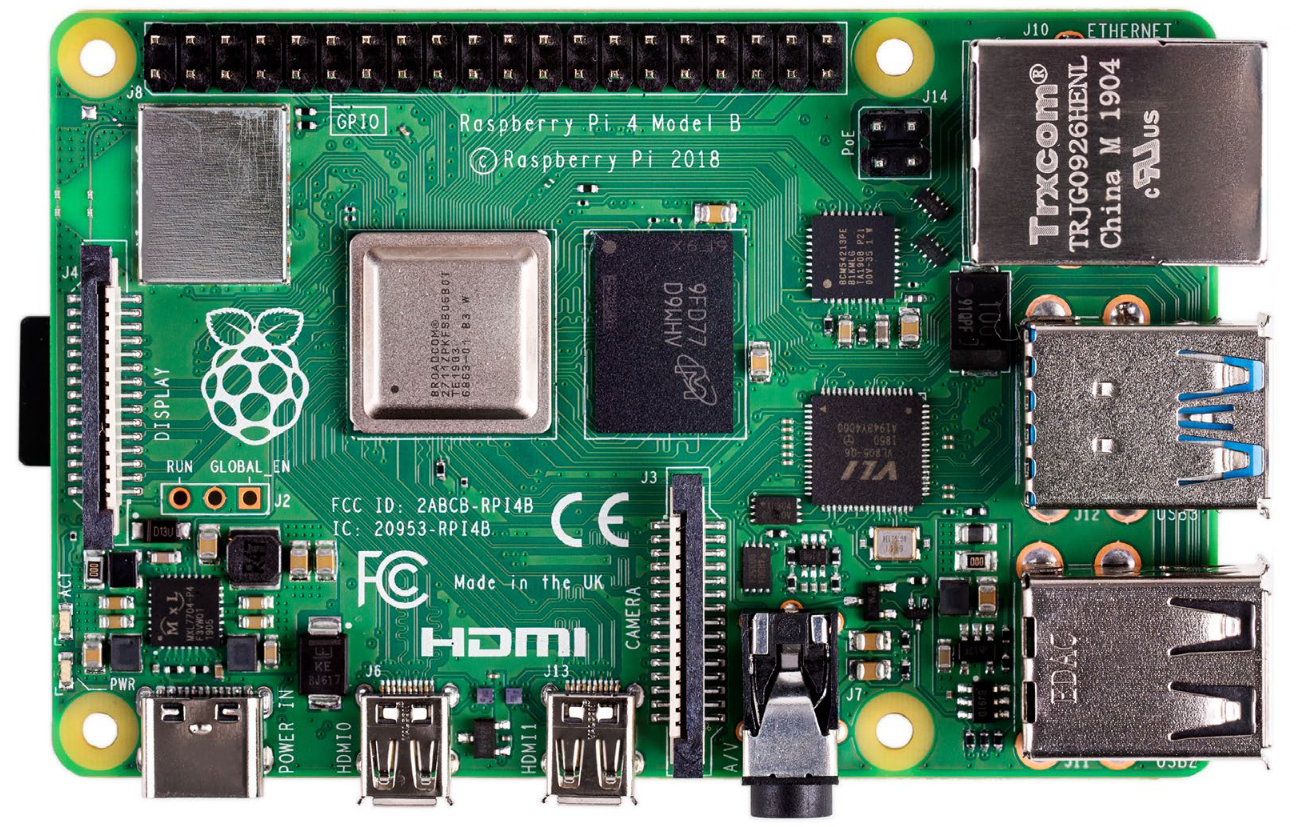
\includegraphics[width=.75\textwidth]{07hw_specification/raspberryPi}
	\caption{Raspberry Pi 4 Model B.}
	\label{fig:rasp}
\end{figure}

%**********************************************************
\subsubsection{\ac{gpio}}

The Raspberry Pi 4 Model B board comes with a standard 40 pin GPIO header, that allows to interface with external peripherals. This GPIO also provides some interface technologys, like UART, I2C or SPI. The GPIO pinout of this board is shown in figure \ref{fig:rasp_pinout} \cite{pinout}.

\begin{figure}[ht]
	\centering
	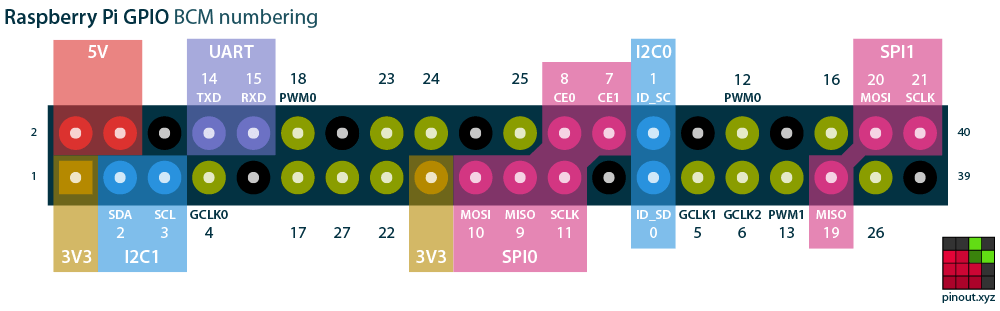
\includegraphics[width=1\textwidth]{07hw_specification/raspberryPi_pinout}
	\caption{Raspberry Pi 4 Model B GPIO Pinout.}
	\label{fig:rasp_pinout}
\end{figure}

%**********************************************************
\subsection{Lamp}

In order to light the streets efficiently, we must use a LED lamp. 

%**********************************************************
\subsection{Luminosity Sensor}

In order to know when is night time, that is, when the light conditions are low, one needs to determine the ambient light conditions, using a module composed by a \ac{ldr} sensor and a LM393 comparator, represented in figure \ref{fig:ldr}. The \ac{ldr} determines the environmental light conditions varying its resistivity. In the table \ref{table:ldr} is shown the LDR Module interface pins. When ambient light intensity does not reach the threshold value (defined by a potentiometer), the module's digital output (DO) is high, and when the ambient light level exceeds the threshold, the module's digital output terminal outputs low.

\begin{figure}[ht]
	\centering
	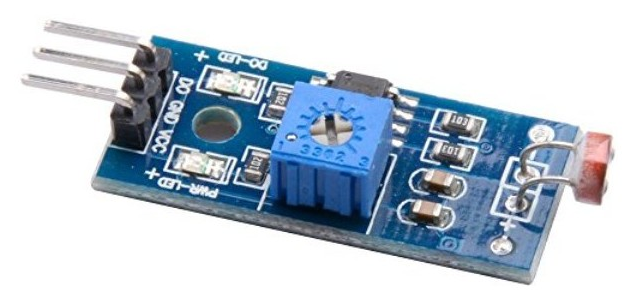
\includegraphics[width=0.70\textwidth]{07hw_specification/ldr}
	\caption{LDR Module.}
	\label{fig:ldr}
\end{figure}

\begin{table}[H]
	\centering
	\resizebox{0.5\columnwidth}{!}{
	\begin{tabular}{||c | c ||} 
		\hline
		\textbf{LDR Module Pin} & \textbf{Board Pin}\\\hline\hline
		VCC & 5 V\\\hline
		DO & Pin 17\\\hline
		GND & GND\\
		\hline
	\end{tabular}
	}		
	
	\caption{LDR Module Interface Pins.}
	\label{table:ldr}
\end{table}

%**********************************************************
\clearpage
\subsection{Motion Detector}
To know when to turn on the light, it is necessary to detect movement in the streets. For this project it is used a motion detector, more specifically a \ac{pir} sensor. The chosen sensor for this purpose was the PIR HC-SR501 that has a supply voltage range of 4,5 - 20 V and a detection range of 7 meters with a 110 degrees angle.

In the table \ref{table:pir} is shown the PIR HC-SR501 interface pins, being the output signal the pin SIGNAL. When no movement is detected, the sensor output is low (0~V), and when movement is detected, the sensor SIGNAL is high (5~V). The sensor has also two potenciometers to adjust the trigger sensitivity and the delay of the trigger signal, between 0,3 seconds and 5 minutes.

\begin{figure}[H]
	\centering
	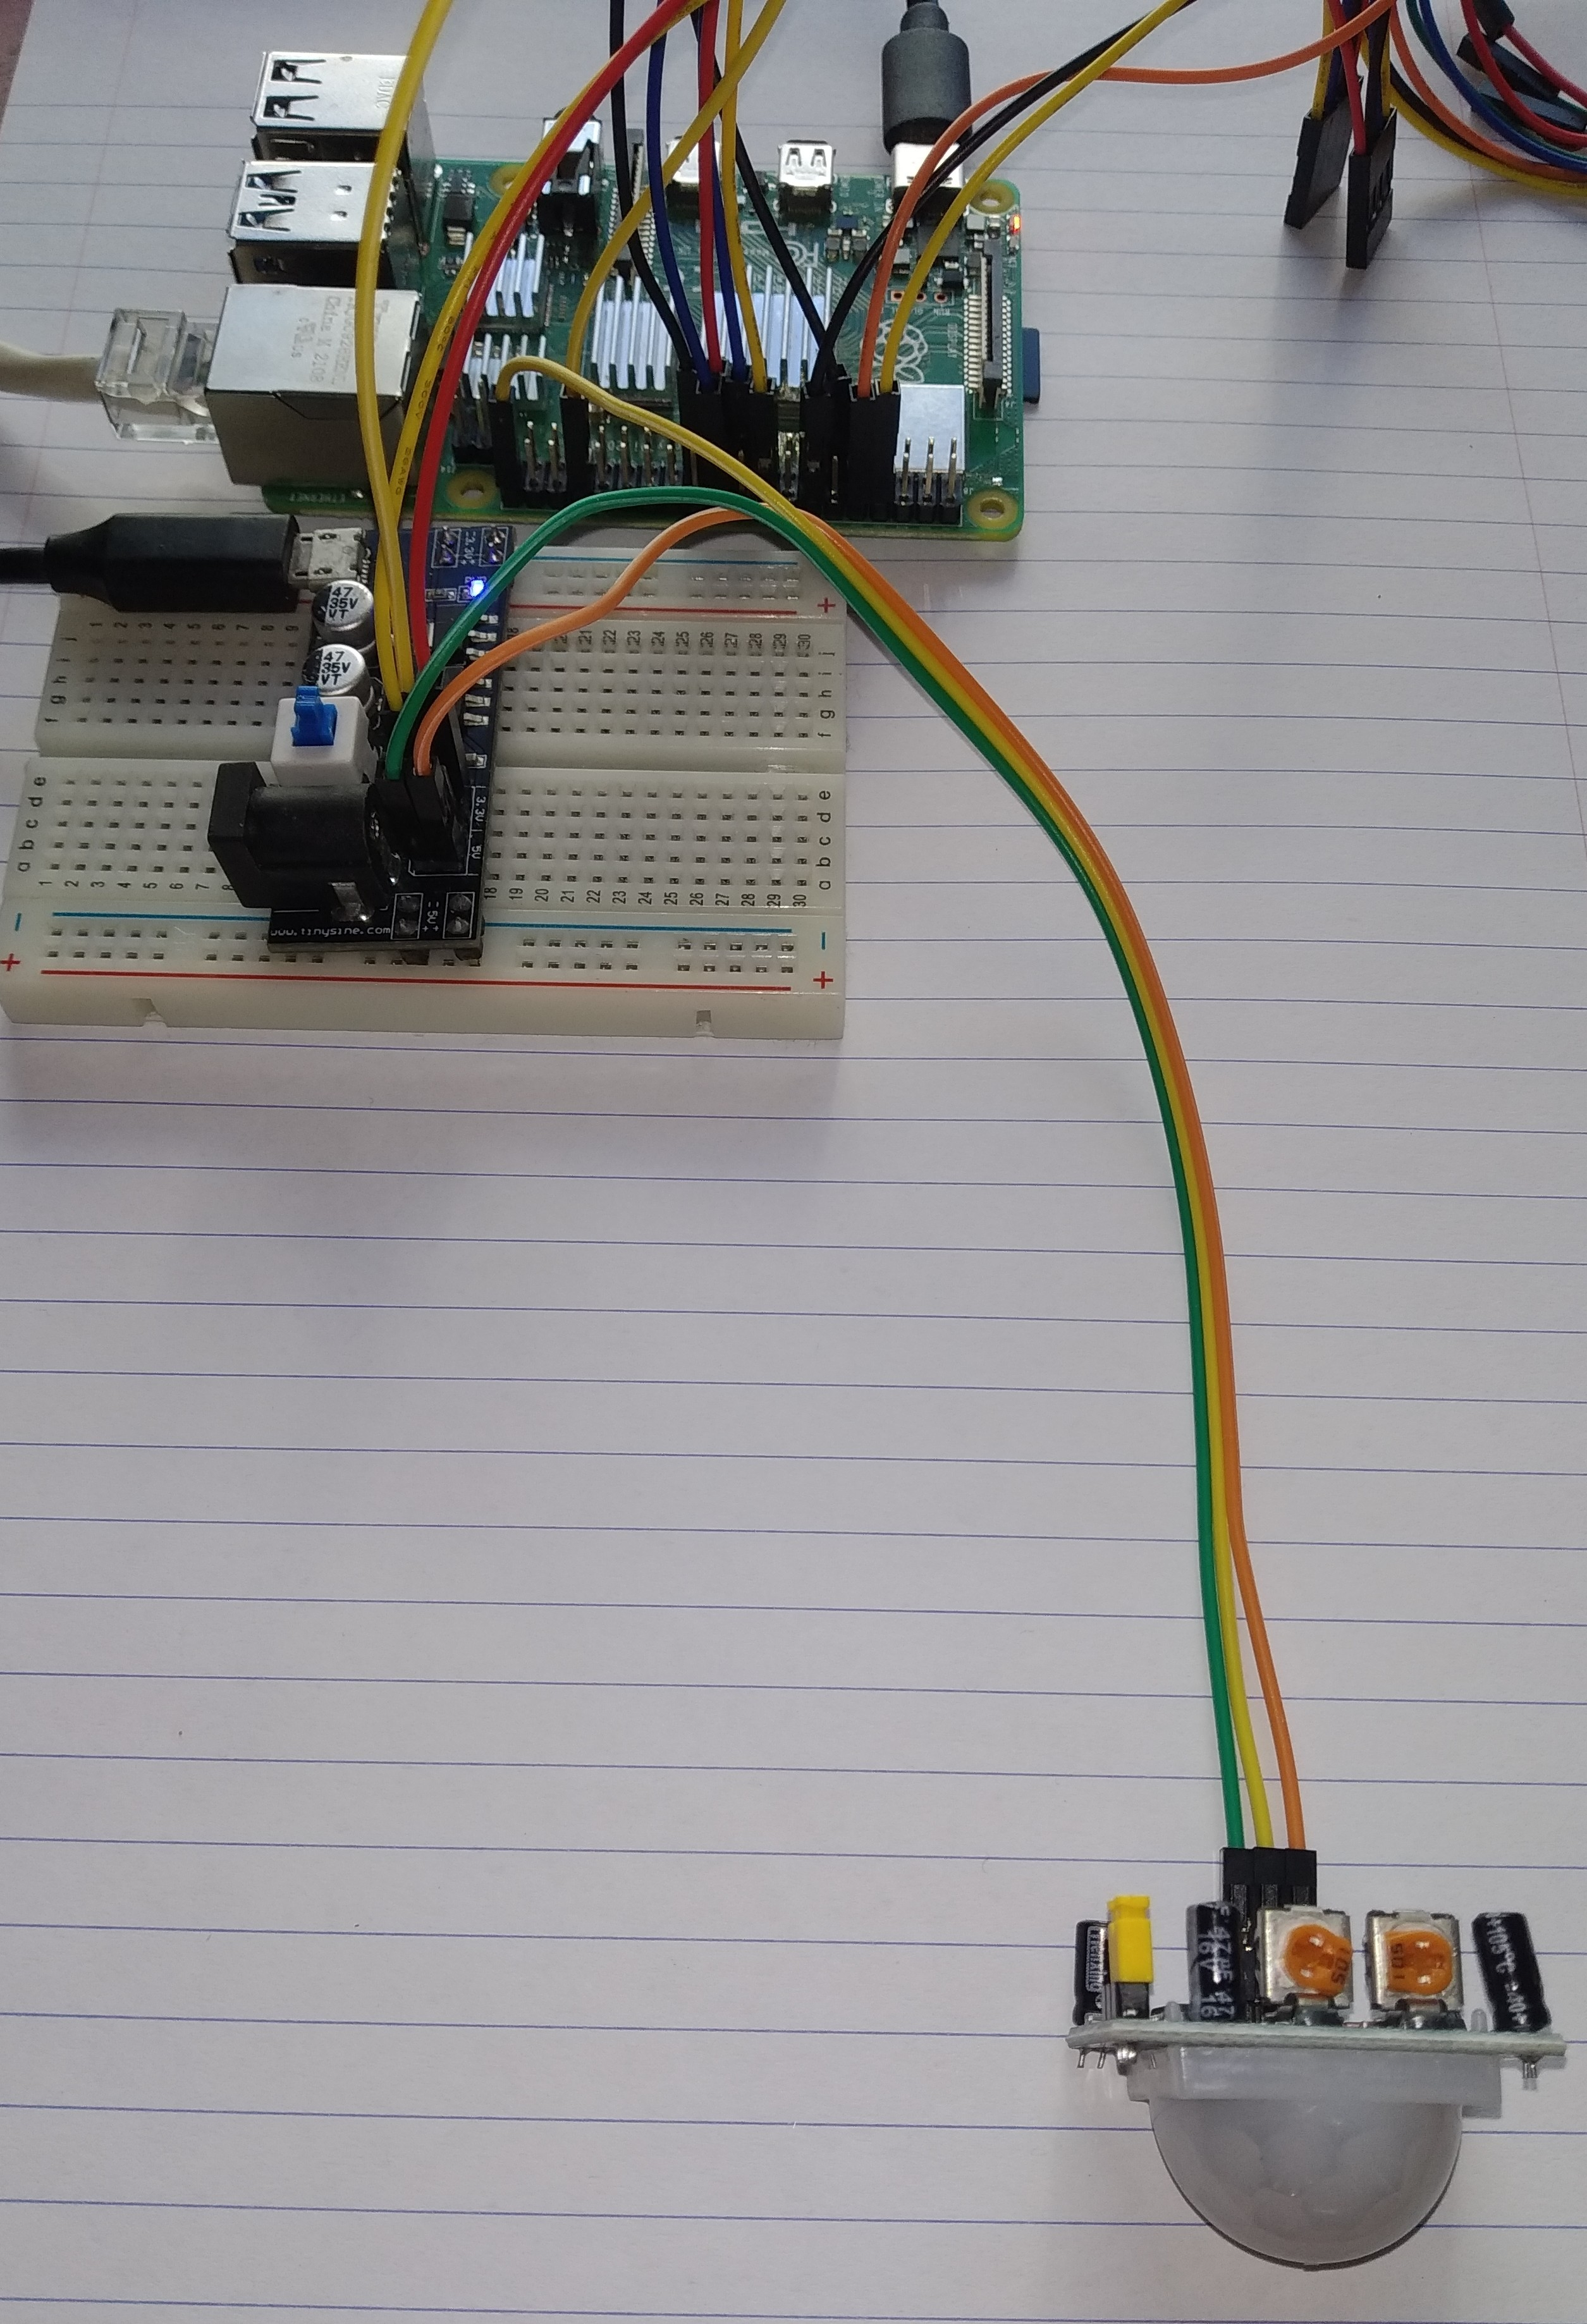
\includegraphics[width=0.70\textwidth]{07hw_specification/pir}
	\caption{PIR Sensor Module.}
	\label{fig:pir}
\end{figure}

\begin{table}[H]
	\centering
	\resizebox{0.5\columnwidth}{!}{
	\begin{tabular}{||c | c ||} 
		\hline
		\textbf{LDR Module Pin} & \textbf{Board Pin}\\\hline\hline
		VCC & 5 V\\\hline
		SIGNAL & Pin 27\\\hline
		GND & GND\\
		\hline
	\end{tabular}
	}		
	
	\caption{PIR Module Interface Pins.}
	\label{table:pir}
\end{table}

%**********************************************************
\subsection{LED Failure Detector}

%**********************************************************
\subsection{Camera}
In order to the detection of available parking spots, it's used a camera, as shown in figure \ref{fig:camera}. This is the Raspberry Pi Camera Module V1, capable of delivering a clear 5 MP resolution image, or 1080p HD video recording at 30fps. \cite{camera}

\begin{figure}[H]
	\centering
	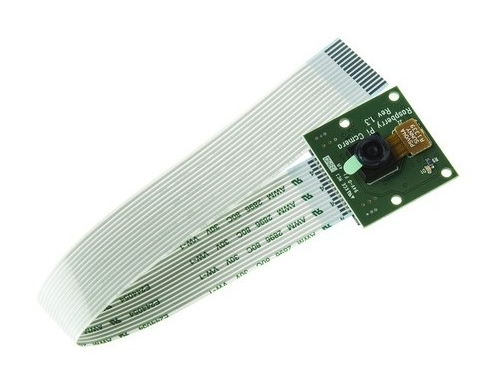
\includegraphics[width=0.6\textwidth]{07hw_specification/camera}
	\caption{Raspberry Pi Camera Module V1.}
	\label{fig:camera}
\end{figure}

\paragraph*{Characteristics}
\begin{itemize}
	\item 5MP OmniVision 5647 sensor;
	\item Fixed focus lens onboard;
	\item Still Picture Resolution: 2592 x 1944;
	\item 15-pin ribbon cable, to the dedicated 15-pin MIPI \ac{csi};
	\item Video recording: Supports 1080p @ 30fps, 720p @ 60fps.
\end{itemize}

\clearpage
\myparagraph{Connection scheme}
This camera module plugs directly into the \ac{csi} connector on the Raspberry Pi, as shown in figure \ref{fig:connect_camera}, through the use of a 15-pin ribbon cable.

\begin{figure}[ht]
	\centering
	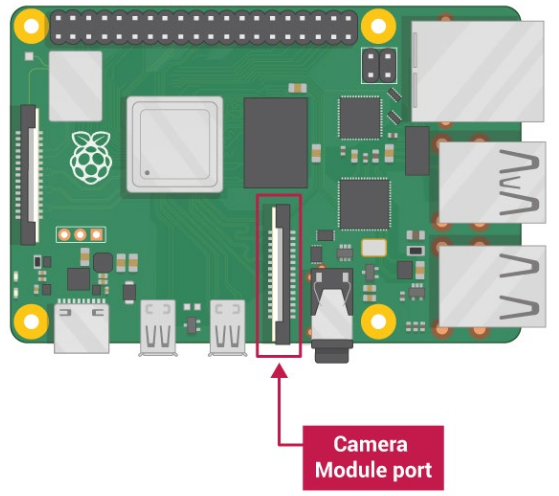
\includegraphics[width=0.60\textwidth]{07hw_specification/connect_camera}
	\caption{Connection scheme: Camera Module.}
	\label{fig:connect_camera}
\end{figure}
%**********************************************************
\clearpage
\subsection{LoRa Module}
To allow each local system to communicate to the gateway, it's used LoRa communication technology, requiring for that a LoRa Module, as the one presented in figure \ref{fig:lora_module}. This module, from Ai-Thinker company, uses SX1278 \ac{ic} from SEMTECH, and works on a 433~MHz frequency, with a range up to 10 km in line of sight. \cite{sx1278} \cite{lora_module}

\begin{figure}[H]
	\centering
	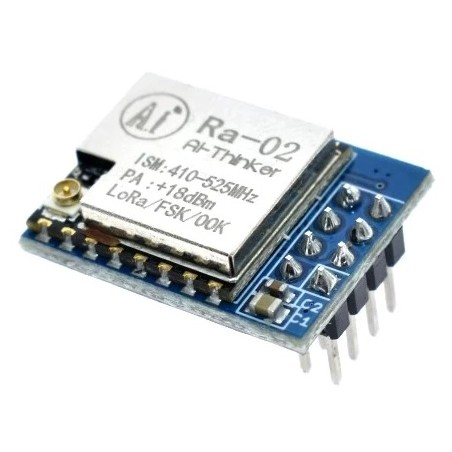
\includegraphics[width=0.5\textwidth]{07hw_specification/lora_module}
	\caption{LoRa Module SX1278 RA-02 433 MHz.}
	\label{fig:lora_module}
\end{figure}

\paragraph*{Characteristics}
\begin{itemize}
	\item LoRa modulation technology (Supports also FSK, GFSK, MSK, GMSK and OOK modulation modes);
	\item Effective Bitrate : 0,018 - 37,5 kbps;
	\item Half-duplex SPI communication;
	\item Programmable bit rates up to 300kbps;
	\item Packet engine with CRC up to 256 bytes;
	\item Small footprint dual-row stamp-hole patch package;
	\item Male U.FL connector to support using of external RF antenna - Diameter: 15,5mm.
\end{itemize}

\begin{table}[H]
	\centering
		\begin{tabular}{|m{5cm}|m{6cm}|}
			\hline
			\textbf{SX1278 RA-02 Pinout} & \textbf{Description}
			\\\hline\hline
		
			VCC & Power in - 3,3 V\\\hline
			GND & Ground\\\hline
			RST & Reset \\\hline
			SCK & SPI clock input\\\hline
			NSS & SPI selected-IN\\\hline
			MISO & SPI data output\\\hline
			MOSI & SPI data input\\\hline
			DIO0 & Digital Input/Output 0\\\hline
		\end{tabular}
	
	\caption{LoRa Module SX1289 RA-02 Pinout Description.}
	\label{table:lora_module_pinout}
\end{table}

In order to achieve longer range and better signal quality in LoRa communication, an antenna may be used, as the one shown in figure \ref{fig:lora_antena}. RF antennas play a critical role in diverting, directing or concentrating radio wave transmission in a particular direction. 

%Antennas that have high gain will enable one to achieve longer range and better signal quality in LoRa communication, but must be aimed specifically in the direction of the receiving antenna. 

\begin{figure}[H]
	\centering
	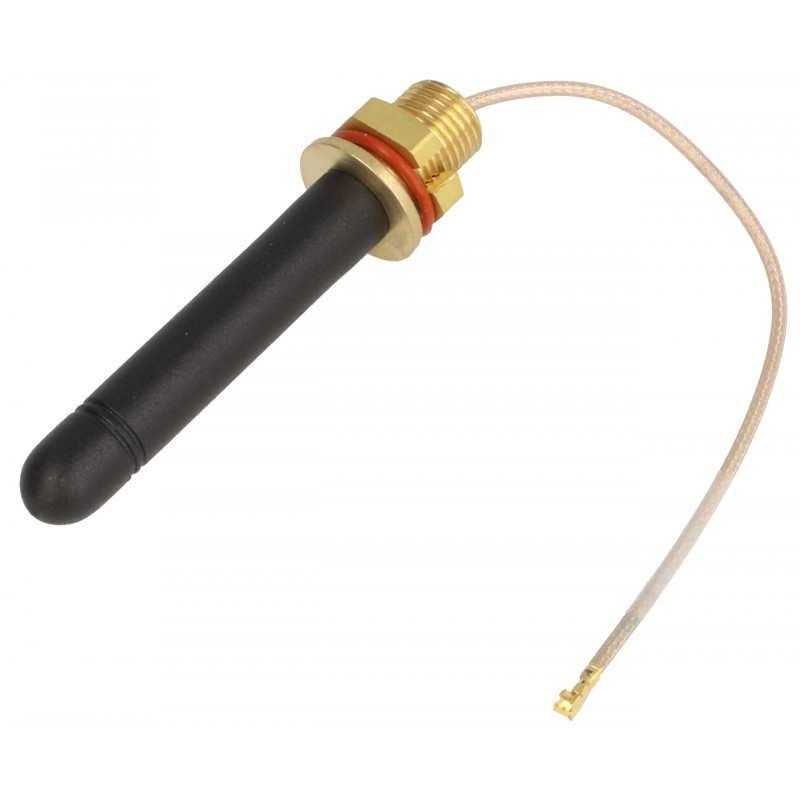
\includegraphics[width=0.40\textwidth]{07hw_specification/lora_antena}
	\caption{RF Antenna 433 MHz.}
	\label{fig:lora_antena}
\end{figure}

\paragraph*{Characteristics}
\begin{itemize}
	\item Frequency: 433,05 - 434,79 MHz;
	\item Antenna gain: 2 dBi;
	\item Connector I-PEX (U.FL) - Diameter: 15,5mm;
	\item Impedance 50 $\Omega$.
\end{itemize}

\myparagraph{Connection scheme}
In table \ref{table:connect_lora} it is shown the connection scheme of the LoRa module to the Raspberry Pi (remember figure \ref{fig:rasp_pinout}). Also keep in mind that the RF antenna is connected directly to the LoRa module, through an U.FL connector.

\begin{table}[H]
	\centering
	\begin{tabular}{|m{5cm}|m{6cm}|}
		\hline
		\textbf{SX1278 RA-02} & \textbf{Raspberry Pi}
		\\\hline\hline
		
		VCC & 3,3 V
		\\\hline
		GND & GND
		\\\hline
		RST & GPIO 4
		\\\hline
		SCK & CLK
		\\\hline
		NSS & SPI0 CE0
		\\\hline
		MISO & SPI0 MISO
		\\\hline
		MOSI & SPI0 MOSI
		\\\hline
		DIO0 & GPIO 17
		\\\hline
	\end{tabular}
	
	\caption{Connection scheme: LoRa Module.}
	\label{table:connect_lora}
\end{table}

%**********************************************************
\subsection{Driver}

%**********************************************************
\subsection{Power Module}
% step-down converter
% industrial power supply

%**********************************************************
\subsection{Hardware review} %?????
% show hardware architecture with all protocols defined in
% each connection